% Copyright (C) 2010 Thomas L. Kula
% All Rights Reserved
%
% See the file LICENSE for license terms.
\documentclass[12pt]{article}
\usepackage{graphicx}
\usepackage{rotating}
\usepackage{fix-cm}
\setlength{\paperwidth}{5.5in}
\setlength{\paperheight}{8.5in}
\setlength{\textheight}{7.45in}
\setlength{\topmargin}{-1.0in}
\setlength{\oddsidemargin}{-0.5in}
\setlength{\evensidemargin}{-0.5in}
\setlength{\textwidth}{4.0in}
\setlength{\parindent}{0in}
\setlength{\parskip}{3mm}
\usepackage[print]{booklet} \nofiles
\source{\magstep0}{5.5in}{8.5in}
\target{\magstep0}{11in}{8.5in}
\setpdftargetpages
\pagestyle{empty}
\begin{document}


\begin{center}
{\fontsize{36}{48}\selectfont \textsc{Haiku a Day }}
\end{center}

\vspace*{3.5cm}

{\fontsize{26}{52}\selectfont 

There --- a hint of spring

Winter, now fading away,

Gives a last hurrah

}

\vspace*{5.0cm}
\begin{center}
{\large{Issue 56: February 2010}} \\[5mm]
{\fontsize{8}{8}\selectfont  \textsc{ St. Joshua Norton Press }} \\[1mm]
{\fontsize{6}{6}\selectfont Mathom House in Midtown \textbar The People's Republic of Ames }
\end{center}


\newpage

I love winter, and cold weather, but there is a point each year when
I long for spring, and nice walks outside, bike rides that aren't
miserable, the farmer's market and fresh produce, and bike polo in 
the outdoors, where it's supposed to be played. After one final
eight inch blast, Winter, I hope, has left Ypsilanti.

--- Thomas

http://kula.tproa.net/had/ \\
kula@tproa.net

Download this and previous HADs at the website, so you can
print out your own (DIY, yeah!) or if you want me to send
you one, send me your address, and maybe a stamp if you
are feeling nice. Or send me something you've made ---
trades always appreciated, postcards are nice too.

\vspace*{2cm}

\newpage

1 February 2010

A reading backlog \\
And yet, I'm filled with boredom \\
Too many choices?

2 February 2010

A pot on the stove \\
For hours on a low heat \\
Contents abubble

3 February 2010

``Ah-ha'' I can say \\
The drowsy morning waking \\
Making my brain work

4 February 2010

Hands soaked in water \\
They get wrinkled and gritty \\
Once dry they're restored

5 February 2010

A bad week ending \\
And a day without working \\
Makes my mood lighter

6 February 2010

A wall of music \\
Solid sound pushing your ears \\
Stops. Quiet deafens

7 February 2010

There's an easy way \\
When you're picking up spilled pins \\
If there's a magnet....


\newpage

8 February 2010

Drip ... drip ... drip ... drip ... drip ... \\
I can not make the sound stop \\
Drip ... drip ... drip ... drip ... drip ...

9 February 2010

Like a soybean sponge \\
Absorbing all kinds of stuff \\
Tofu, you suck well

10 February 2010

Calm in a large space \\
Squished becomes hot and angry \\
Compression of gas

11 February 2010

Quarter explosion \\
Coins spilling across the floor \\
Collect for laundry

12 February 2010

Swaying in the breeze \\
A slender wire moving \\
Makes a twisty path

13 February 2010

I wish for pickles \\
And yet no pickles arrive \\
What's wrong with this world?

14 February 2010

Some nights I go on \\
Wikipedia wanders \\
Where weird paths emerge

\newpage

15 February 2010

The world, upside down \\
Different, exciting, new \\
There yet never there

16 February 2010

Simple yet complex \\
Can openers mesmerise \\
My beans are open

17 February 2010

High on Sherzer Hall \\
Look down on Ypsilanti \\
Absorb its beauty

18 February 2010

Soft in the distance \\
I hear a car horn honking \\
Over and over

19 February 2010

Tidy grows messy \\
The neverending battle \\
Fought against clutter

20 February 2010

A day of errands \\
When finished gives a sense of \\
Productivity

21 February 2010

No wheel, no polo \\
Instead, some photography \\
I'm trapping photons

\newpage

22 February 2010

With heavy snowfall \\
My bloodpressure rises as  \\
Idiots abound

23 February 2010

There in a window \\
``As Seen On TV Sold Here'' \\
That's a product now?

24 February 2010

The life of a mug \\
Full of hot, cold, maybe soup \\
The mug stays the same

25 February 2010

The sun does not rise \\
It's caused by the Earth spinning \\
Yet I see a rise

26 February 2010

Go away devil \\
The little imp in my head \\
A headache headache

27 February 2010

Song stuck in my head \\
A pleasant tune but no words \\
It is maddening

28 February 2010

February done? \\
Where the hell has this month gone? \\
Feel cheated somehow.

\newpage

\begin{center}
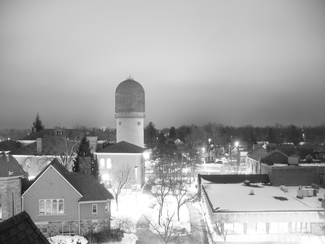
\includegraphics{ypsi-from-sherzer.jpg} \\[1cm]

Ypsilanti from the top of Sherzer Hall, EMU  

\small{{\tt http://kula.tproa.net/photos/2010/20100217-sherzer-hall/ }}

\end{center}

\newpage

\thispagestyle{empty}
\vspace*{14cm}
\begin{sideways}
\Large{Thomas L. Kula}
\end{sideways}
\begin{sideways}
\Large{PO Box 980461}
\end{sideways}
\begin{sideways}
\Large{Ypsilanti MI 48198}
\end{sideways}


\end{document}


